\documentclass[../../main.tex]{subfiles}

\begin{document}
\problem{18}
\begin{wts}
Select the first DNS packet in your trace. From this packet, determine the header fields of UDP.
\end{wts}
\begin{proof}
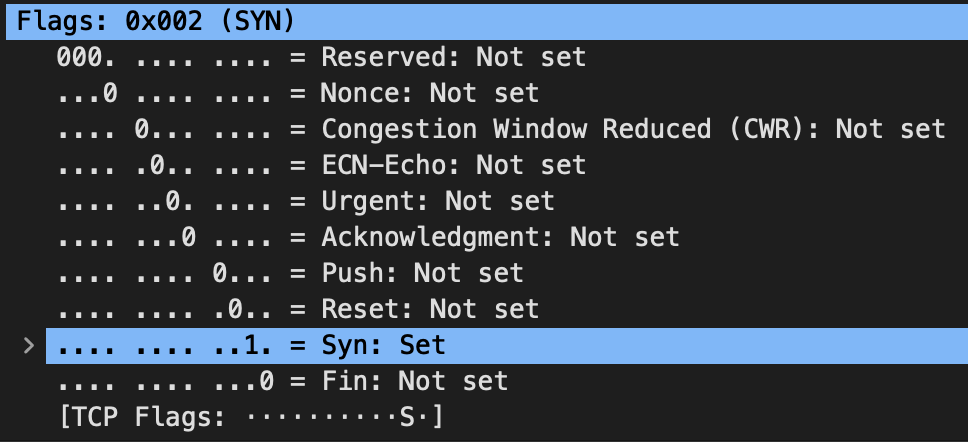
\includegraphics[width=\textwidth]{subfiles/images/ECSE_308_Lab_5_1_SUPA_PAGE1_1_Image28.png
}
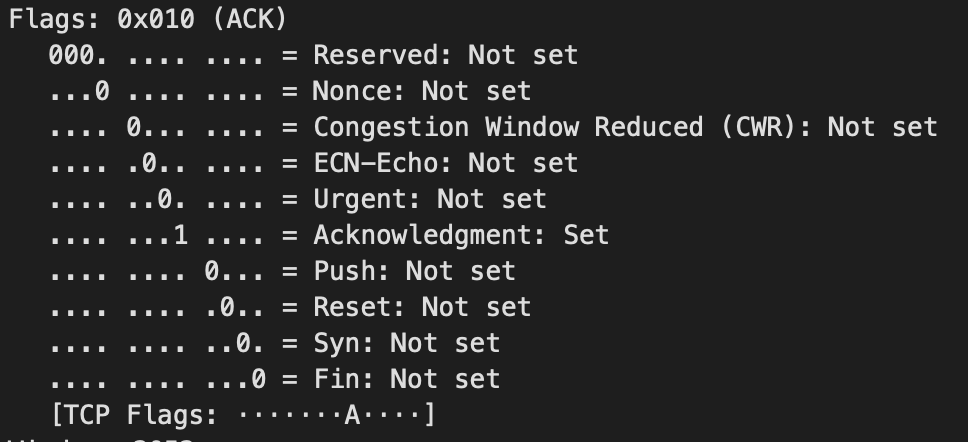
\includegraphics[width=\textwidth]{subfiles/images/ECSE_308_Lab_5_1_SUPA_PAGE1_3_Image30.png}
\subfile{./Folland/Theorem4_25.tex}
\end{proof}

\begin{wts}
   Find the limit points for the following subsetes of $\real^2$.
   \begin{enumalpha}
        \item $\{(m,n),\,m,n\in\mathbb{Z}\}$,
        \item $\{(p,q),\,p,q\in\mathbb{Q}\}$,
        \item $\{(m/n,n^{-1}),\,m,n\in\mathbb{Z},\,n\neq 0\}$,
        \item $\{(n^{-1}+m^{-1},0),\,m,n\in\mathbb{Z}\setminus\{0\}\}$
   \end{enumalpha}
\end{wts}
\begin{proof}[Proof for Part A]
    Let $S=\{(m,n),\,m,n\in\mathbb{Z}\}$, and we claim that $\acc{S}=\varnothing$. Suppose by contradiction that $\acc{S}\neq\varnothing$, for any $(a,b)\in\acc{S}$, we can always take $\varepsilon=2^{-1}>0$, and this induces some $(m,n)\in S$ with 
    \[
        |a-m|^2+|b-n|^2<2^{-2}\iff \begin{cases}|a-m|<2^{-1}\\
        |b-n|<2^{-1}\end{cases}
    \]
    We claim that this $(m,n)\in S$ is unique, indeed, if there exists some $(m',n')\in S$ such that $d(m,m')\geq 1$ and $d(n,n')\geq 1$, by the triangle inequality we have
    \[
    1\leq d(m,m')\leq d(a,m) + d(a,m')\implies 2^{-1}\leq d(a,m')
    \]
    Since $(m,n)$ is unique, we can conclude that 
    \[
        (m,n)\in \bigcap_{n\geq 1} V_{2^{-n}}(a,b)
    \]
    This is equivalent to saying that for every $\varepsilon>0$, by the Archimedean Property, $d((m,n),(a,b))<2^{-n}<\varepsilon$, therefore $(m,n)=(a,b)\in S$. It follows that $V_{2^{-1}}(m,n)\cap S\setminus\{(m,n)\}=\varnothing$, $(m,n)$ cannot be an accumulation point of $S$. Thus $\acc{S}=\varnothing$.
\end{proof}

\begin{proof}[Proof of Part B]
    Let $S = \{(p,q),\, p,q\in\mathbb{Q}\}$, we claim that $\acc{S}=\real^2$. Note that $\acc{S}\subseteq\real^2$ implicitly. It suffices to show the reverse estimate. We accomplish this by first fixing an element $(x,y)\in\real^2$. By the density of $\mathbb{Q}$ in $\real$, there exists two sequences $x_n\to x$ and $y_n\to y$ where $x_n,y_n\in\mathbb{Q}$. For any ${\varepsilon 2^{-1/2}}>0$, $x_n\in V_{\varepsilon 2^{-1/2}}(x)$ and $y_n\in V_{\varepsilon 2^{-1/2}}(y)$ eventually, combining the two we get
    \[
       \begin{cases}
        |x_n-x|<{\varepsilon 2^{-1/2}}\\
        |y_n-y|<{\varepsilon 2^{-1/2}}
       \end{cases}
       \implies
       \begin{cases}
        |x_n-x|^2<{\varepsilon^2 2^{-1}}\\
        |y_n-y|^2<{\varepsilon^2 2^{-1}}
       \end{cases}
       \implies |x_n-x|^2+|y_n-y|^2<\varepsilon^2
    \]
    Taking square roots on both sides finishes the proof.
\end{proof}
\begin{remark}
    We used the fact that $\real^2$ is first countable, and $(x,y)\in\acc{S}\iff$ there exists a sequence in $S$ that converges to $(x,y)$. To show that $\real^2$ is first countable, fix any $\vec{v}\in\real^2$, and take the family of open balls centered at $\vec{v}$ with rational radius.
\end{remark}

\begin{proof}[Proof of Part C]
    Let $S=\{(m/n,1/n),\,m,n\in\mathbb{Z},\,n\neq 0\}$, and we claim that $\acc{S}=\{(a,0),\,a\in\real\}$. Fix an element  $(a,0)\in A$, where $A$ denotes the right member of the previous equality. By the density $\mathbb{Q}$ in $\real$, there exists a sequence $\{q_n\}\subseteq \mathbb{Q}$ with $q_n\to a$. We will modify this $q_n$ to produce a sequence $\{(x_n,y_n)\}\subseteq S$ that converges to $(a,0)$.
    \begin{itemize}
        \item It suffices to assume that $|q_n-a|<(2^{-n})2^{-1/2}$, otherwise we can choose a subsequence of $q_n$ that satisfies this property and relabel $q_n$, then
        \item For every $n\geq 1$, $q_n$ induces some $q_n=m_n/d_n$, by the Archimedean Property, and since we can assume that $d_n>0$; we can always find some corresponding $k_n\in\nat^+$ so large that
        \[
            (k_n)^{-1}<(2^{-n})2^{-1/2}d_n
        \]
        \item Let $x_n = k_nm_n/k_nd_n$, where $k_nm_n\in\mathbb{Z}$, and $k_nd_n\in\nat^+\subseteq\mathbb{Z}\setminus\{0\}$.
        \item And define $y_n=(k_nd_n)^{-1}$, so that $(x_n,y_n)\in S$ for every $n\geq 1$.
        \item To show convergence, fix some $\varepsilon>0$, and eventually $\varepsilon<2^{-n}$ for $n$ large enough, hence
        \[
            \biggl(|x_n-a|^2+|y_n-0|^2\biggr)^{1/2}<2^{-n}<\varepsilon
        \]
    \end{itemize}
    Let us agree to define 
    \begin{itemize}
        \item $W = \{(a,0),\,a\in\mathbb{R}\}$, 
        \item $\mathbb{Z}^*=\mathbb{Z}\setminus\{0\}$,
    \end{itemize}
    We wish to show $W^c\subseteq \acc{S}^c$. Suppose on the contrary that there exists some $(a,b)\in W^c$ so that $b\neq 0$. We have three cases to consider.
    
    \begin{enumerate}
        \item If $b=(n)^{-1}$ for some $n\in\mathbb{Z}^*, |n|\geq 2$, fix 
        \[
            \varepsilon=\min\biggl\{|(n+1)^{-1}-n^{-1}|,|(n-1)^{-1}-n^{-1}|\biggr\}2^{-1}
        \]
        Then $\varepsilon>0$ is obvious, and suppose that there exists some $(mk^{-1},k^{-1})\in S$ with
        \[\begin{cases}
            |mk^{-1}-a|<\varepsilon\\
            |k^{-1}-b|<\varepsilon
        \end{cases}\]
        Focusing on the second inequality, we get
        \[\begin{cases}
            |k^{-1}-n^{-1}|<|(n+1)^{-1}-n^{-1}|\\
            |k^{-1}-n^{-1}|<|(n-1)^{-1}-n^{-1}|
        \end{cases}\]
        Clearly this forces $k=n$, and resuming from the first inequality, 
        \begin{align*}
            |mk^{-1}-a|<\varepsilon&\iff |mn^{-1}-a|<\varepsilon\\
            &\iff -\varepsilon|n|+an<m<+\varepsilon|n|+an
        \end{align*}
        Since the permissible values for $m\in\mathbb{Z}$ lie in a finite interval, there are only finitely many $m$, and this neighbourhood contains only finitely many points of $S$, therefore $(a,b)\notin \acc{S}$.
        %
        \item If $b=(n)^{-1}$ for some $n\in\zs, |n|=1$, then let us take $\varepsilon=4^{-1}$. It is clear that 
        \[
            V_{4^{-1}}(b)\bigcap\{n^{-1},\,n\in\zs\}=\{b^{-1}\}
        \]
        Then $V_{4^{-1}}(b)\cap S$ is finite, and $(a,b)\notin\acc{S}$.
        %
        \item If $b\neq(n)^{-1}$ for all $n\in\zs$, then choose $\varepsilon=|b|2^{-1}$. Suppose that $b>0$, then by the Archimedean Property, there exists an $n\in\nat^+$ so large that $n^{-1}<b/2<b$. So that the set $E=\{n\in\nat^+, n^{-1}<b/2\}$ is not empty. Let $N$ be the least member of that set, then it follows that for every $n<N$, $n\in\nat^+$ means that $n^{-1}\geq |b|/2$. Let $\delta=\min\{|n^{-1}-b|,\,n\notin E^c\}>0$, and relabel $\varepsilon=\min\{|b|/2,\delta\}>0$. It is trivial to verify that no $k\in\zs$ can satisfy $|k^{-1}-b|<\varepsilon$. Therefore, $V_\varepsilon(a,b)\cap S=\varnothing$, and $(a,b)\notin\acc{S}$, and the case for when $b<0$ follows immediately, and it is left as an exercise.
    \end{enumerate}
\end{proof}\newpage
\begin{proof}[Proof of Part D]
    We claim that if $S=\{(n^{-1}+m^{-1},0),\,n,m\in\mathbb{Z}\setminus\{0\}\}$, then $\acc{S}=W$, where $W = \{(k^{-1},0),k\in\zs\}$. We first show that $W\subseteq \acc{A}$. Fix some $(k^{-1},0)\in W$, then for any $\varepsilon>0$, by the Archimedean property, there exists some $n\in\nat^+$ so large that $n^{-1}<\varepsilon$, and therefore
    \[
        |k^{-1}-(k^{-1}+n^{-1})|=|n^{-1}|<\varepsilon
    \]
    Conversely, suppose that $(a,b)\in\acc{S}$, then the remainder of the proof is divided into three steps.
    \begin{enumerate}
        \item We wish to show that $b=0$, indeed, if $b\neq 0$, then for any $(m^{-1}+n^{-1},0)\in S$, 
        \[
            0<|b|\leq \biggl(|b-0|^2+|a-(m^{-1}+n^{-1})|\biggr)^{1/2}
        \]
        the resulting contradiction follows if we choose $\varepsilon=|b|/2$.
        \item Now suppose that $a>0$, and $b=0$, then by the Archimedean Property, there exists some $A\in \nat^+$ with\[a\leq 1\iff a^{-1}\geq 1\implies A>a^{-1}>A-1\geq 1\]
        \item Now for this $A\geq 2$, let us write 
        \[\lambda = \min\biggl\{|A^{-1}-a|,|(A-1)^{-1}-a|\biggr\}2^{-1}\]
        For the sake of completness, notice also that $a$ sits in between $A^{-1}$ and $(A-1)^{-1}$, 
        \[
            \dfrac{1}{A}<a<\dfrac{1}{A-1}
        \]
        \item Since $(a,b)\in\acc{S}$, and we have ruled out the possibility of $b\neq 0$, we can treat $S=\{m^{-1}+n^{-1},\,m,n\in\zs\}$, and it suffices to find a sequence $\{x_n\}\subseteq S$ such that if $a\in\acc{S}$ (with the new, relabelled $S$), with $x_n\to a\implies a=k^{-1}$ for some $k\in\zs$.
        \item Choose $x_1$ using $\lambda$:\[x_1\in S,\quad0<|a-x_1|<\lambda\]
        \item Choose the remainder of the sequence inductively with
        \[
          x_n\in S,\quad 0<|a-x_n|<|a-x_{n-1}|2^{-1},  
        \]
        \item Observe that all the elements in the above sequence are distinct, and each $x_n$ induces some $m_n,n_n\in\zs$, such that
        \[x_n=m_n^{-1}+n_n^{-1}\]
        From this, we know that it cannot be the case that both $m_n$, and $n_n$ have bounded ranges. Since we have infinitely many distinct terms in $x_n$.
        \item More is true, we cannot have both $m_n\to\pm\infty$ and $n_n\to\pm\infty$, since this would mean that $x_n\to 0=a\neq 0$.
        \item Hence, we can make the assumption that only $n_n\to \pm\infty$ with $m_n$ being bounded.
        \item For the sequence $x_n$ to converge at all, $m_n$ must become eventually constant for some $m_n=k\in\zs$, given that $n_n\to\pm\infty$ and\[x_n=\biggl(\dfrac{1}{m_n}+\dfrac{1}{n_n}\biggr)\to \dfrac{1}{m_n}\to\dfrac{1}{k},\quad k\in\zs\] 
        \item Therefore $a=k^{-1}$, and $(a,0)\in W$ (our original $W$).
        \item The case for when $a<0$ is similar. Replace $a$ with $a'=-a>0$, and repeat the steps. Since $-k\in\zs$ for any $k\in \zs$, the proof is complete.
    \end{enumerate}
\end{proof}
\end{document}